% Options for packages loaded elsewhere
\PassOptionsToPackage{unicode}{hyperref}
\PassOptionsToPackage{hyphens}{url}
%
\documentclass[
  ignorenonframetext,
]{beamer}
\usepackage{pgfpages}
\setbeamertemplate{caption}[numbered]
\setbeamertemplate{caption label separator}{: }
\setbeamercolor{caption name}{fg=normal text.fg}
\beamertemplatenavigationsymbolsempty
% Prevent slide breaks in the middle of a paragraph
\widowpenalties 1 10000
\raggedbottom
\setbeamertemplate{part page}{
  \centering
  \begin{beamercolorbox}[sep=16pt,center]{part title}
    \usebeamerfont{part title}\insertpart\par
  \end{beamercolorbox}
}
\setbeamertemplate{section page}{
  \centering
  \begin{beamercolorbox}[sep=12pt,center]{part title}
    \usebeamerfont{section title}\insertsection\par
  \end{beamercolorbox}
}
\setbeamertemplate{subsection page}{
  \centering
  \begin{beamercolorbox}[sep=8pt,center]{part title}
    \usebeamerfont{subsection title}\insertsubsection\par
  \end{beamercolorbox}
}
\AtBeginPart{
  \frame{\partpage}
}
\AtBeginSection{
  \ifbibliography
  \else
    \frame{\sectionpage}
  \fi
}
\AtBeginSubsection{
  \frame{\subsectionpage}
}
\usepackage{lmodern}
\usepackage{amsmath}
\usepackage{ifxetex,ifluatex}
\ifnum 0\ifxetex 1\fi\ifluatex 1\fi=0 % if pdftex
  \usepackage[T1]{fontenc}
  \usepackage[utf8]{inputenc}
  \usepackage{textcomp} % provide euro and other symbols
  \usepackage{amssymb}
\else % if luatex or xetex
  \usepackage{unicode-math}
  \defaultfontfeatures{Scale=MatchLowercase}
  \defaultfontfeatures[\rmfamily]{Ligatures=TeX,Scale=1}
\fi
% Use upquote if available, for straight quotes in verbatim environments
\IfFileExists{upquote.sty}{\usepackage{upquote}}{}
\IfFileExists{microtype.sty}{% use microtype if available
  \usepackage[]{microtype}
  \UseMicrotypeSet[protrusion]{basicmath} % disable protrusion for tt fonts
}{}
\makeatletter
\@ifundefined{KOMAClassName}{% if non-KOMA class
  \IfFileExists{parskip.sty}{%
    \usepackage{parskip}
  }{% else
    \setlength{\parindent}{0pt}
    \setlength{\parskip}{6pt plus 2pt minus 1pt}}
}{% if KOMA class
  \KOMAoptions{parskip=half}}
\makeatother
\usepackage{xcolor}
\IfFileExists{xurl.sty}{\usepackage{xurl}}{} % add URL line breaks if available
\IfFileExists{bookmark.sty}{\usepackage{bookmark}}{\usepackage{hyperref}}
\hypersetup{
  pdftitle={Charitable Giving, Tax Reform, and Government Efficiency},
  hidelinks,
  pdfcreator={LaTeX via pandoc}}
\urlstyle{same} % disable monospaced font for URLs
\newif\ifbibliography
\usepackage{longtable,booktabs}
\usepackage{calc} % for calculating minipage widths
\usepackage{caption}
% Make caption package work with longtable
\makeatletter
\def\fnum@table{\tablename~\thetable}
\makeatother
\setlength{\emergencystretch}{3em} % prevent overfull lines
\providecommand{\tightlist}{%
  \setlength{\itemsep}{0pt}\setlength{\parskip}{0pt}}
\setcounter{secnumdepth}{-\maxdimen} % remove section numbering
\setbeamertemplate{navigation symbols}{}
\setbeamertemplate{footline}[page number]

\usepackage{bookmark}
\usepackage{booktabs}

\usepackage{xltxtra} 
\usepackage{zxjatype} 
\usepackage[ipa]{zxjafont} 
\ifluatex
  \usepackage{selnolig}  % disable illegal ligatures
\fi

\newlength{\cslhangindent}
\setlength{\cslhangindent}{1.5em}
\newlength{\csllabelwidth}
\setlength{\csllabelwidth}{3em}
\newenvironment{CSLReferences}[3] % #1 hanging-ident, #2 entry spacing
 {% don't indent paragraphs
  \setlength{\parindent}{0pt}
  % turn on hanging indent if param 1 is 1
  \ifodd #1 \everypar{\setlength{\hangindent}{\cslhangindent}}\ignorespaces\fi
  % set entry spacing
  \ifnum #2 > 0
  \setlength{\parskip}{#2\baselineskip}
  \fi
 }%
 {}
\usepackage{calc} % for \widthof, \maxof
\newcommand{\CSLBlock}[1]{#1\hfill\break}
\newcommand{\CSLLeftMargin}[1]{\parbox[t]{\maxof{\widthof{#1}}{\csllabelwidth}}{#1}}
\newcommand{\CSLRightInline}[1]{\parbox[t]{\linewidth}{#1}}
\newcommand{\CSLIndent}[1]{\hspace{\cslhangindent}#1}

\title{Charitable Giving, Tax Reform, and Government Efficiency}
  \author{ Hiroki Kato\(^1\)\and Tsuyoshi Goto\(^2\)\and Yong-Rok Kim\(^3\)}
  \institute{\(^1\)Osaka University\and\(^2\)Chiba University\and\(^3\)Kobe University}
\date{2021/02/03}

\begin{document}
\frame{\titlepage}

\begin{frame}
\end{frame}

\hypertarget{introduction}{%
\section{Introduction}\label{introduction}}

\begin{frame}{Background of South Korea Tax Reform}
\protect\hypertarget{background-of-south-korea-tax-reform}{}
To investigate the price effect, we use the 2014 tax reform in the South Korea
(Bursztyn and Jensen, 2017).

\begin{itemize}
\tightlist
\item
  Before 2014, tax deduction was adopted to subsidize charitable donation behavior.
\item
  After 2014, tax credit have been adopted.
\end{itemize}

The main difference is that tax credits reduce taxes directly, while tax deductions indirectly lower the tax burden by decreasing the taxpayer's marginal tax rate, which increases with gross income
\end{frame}

\hypertarget{data}{%
\section{Data}\label{data}}

\begin{frame}{National Survey of Tax and Benefit (NaSTaB)}
\protect\hypertarget{national-survey-of-tax-and-benefit-nastab}{}
\begin{itemize}
\tightlist
\item
  The Korea Institute of Taxation and Finance implements the financial panel survey to study the tax burden of households and the benefits that households receive from goverment.
\item
  The subjects of this survey are general household and household members living in 15 cities and provinces nationwide.
\item
  This survey is based on a face-to-face interview. If it is difficult for investigators to meet subjects, another family member answers on behalf of him.
\item
  Survey items: Annual taxable income (last year), charitable donations (last year), trust for politicians (5-Likert scale), and other covariates (age, education, gender etc.).
\item
  Survey period: 2008 \textasciitilde{} 2019

  \begin{itemize}
  \tightlist
  \item
    We use survey data after 2013 to focus on tax policy change in 2014.
  \end{itemize}
\end{itemize}
\end{frame}

\begin{frame}{Time Series of Chariable Giving}
\protect\hypertarget{time-series-of-chariable-giving}{}
\begin{figure}

{\centering 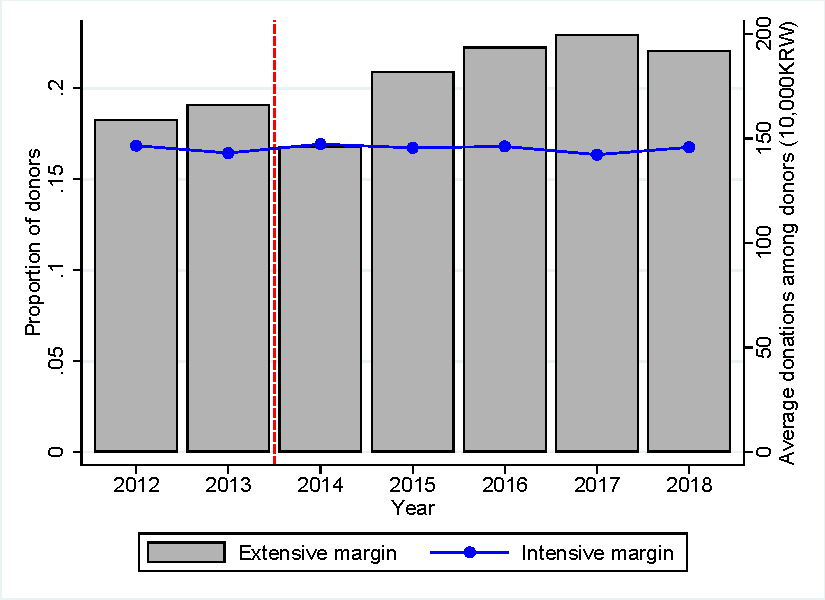
\includegraphics[width=0.9\linewidth]{C:/Users/katoo/Desktop/NASTAB/_assets/SummaryOutcome} 

}

\caption{Proportion of Donors and Average Donations among Donors}\label{fig:unnamed-chunk-1}
\end{figure}
\end{frame}

\begin{frame}{Summary Statistics of Covariates}
\protect\hypertarget{summary-statistics-of-covariates}{}
\begin{table}

\caption{\label{tab:kableSummaryCovariate}Summary Statistics of Covariates}
\centering
\begin{tabular}[t]{lcccc}
\toprule
 & 2012 & 2013 & 2014 & 2015\\
\midrule
Female & 0.51 & 0.51 & 0.52 & 0.52\\
Age & 38.39 & 39.10 & 39.67 & 40.51\\
Annual taxable income & 1699.86 & 1764.04 & 1838.76 & 1872.54\\
University graduate & 0.28 & 0.28 & 0.29 & 0.30\\
High school graduate & 0.30 & 0.30 & 0.31 & 0.31\\
\#.Respondents & 14138 & 13984 & 13787 & 13524\\
\#.Households & 4756 & 4807 & 4819 & 4832\\
\bottomrule
\end{tabular}
\end{table}
\end{frame}

\begin{frame}{Summary Statistics of Covariates (Cont'd)}
\protect\hypertarget{summary-statistics-of-covariates-contd}{}
\begin{table}

\caption{\label{tab:kableSummaryCovariate2}Summary Statistics of Covariates (Continued)}
\centering
\begin{tabular}[t]{lccc}
\toprule
 & 2016 & 2017 & 2018\\
\midrule
Female & 0.52 & 0.52 & 0.52\\
Age & 41.07 & 41.89 & 42.55\\
Annual taxable income & 1906.91 & 1951.55 & 2039.47\\
University graduate & 0.31 & 0.33 & 0.34\\
High school graduate & 0.31 & 0.31 & 0.31\\
\#.Respondents & 13238 & 12963 & 12795\\
\#.Households & 4790 & 4770 & 4765\\
\bottomrule
\end{tabular}
\end{table}
\end{frame}

\begin{frame}{What is Giving Price?}
\protect\hypertarget{what-is-giving-price}{}
Consider allocation between private consumptions (\(x_i\)) and charitable giving (\(g_i\)).
Let \(y_i\) be pre-tax total income.
Then, the budget constraint is

\[
    x_i + g_i = y_i - T_i(y_i, g_i),
\]

where \(T_i\) is tax amount depending on the pre-tax income and charitable giving.
\end{frame}

\begin{frame}{Determination of Tax Amount}
\protect\hypertarget{determination-of-tax-amount}{}
Tax deduction reduces taxable income by giving, that is,

\[
    T_i = \tau(y_i - g_i) \cdot (y_i - g_i),
\]

where \(\tau(\cdot)\) is the marginal income tax rate which is determined by \(y_i - g_i\).

Tax credit reduces tax amount directly, that is,

\[
    T_i = \tau(y_i)\cdot y_i - m g_i,
\]

where \(m \in [0, 1]\) is the tax credit rate.
\end{frame}

\begin{frame}{Derive Giving Price}
\protect\hypertarget{derive-giving-price}{}
Under the tax deduction system, the budget constraint is

\[
    x_i + [1 - \tau(y_i - g_i)]g_i = [1 - \tau(y_i - g_i)] y_i.
\]

Thus, the giving price of tax deduction system is \(p_i^{d} = 1 - \tau(y_i - g_i)\).

Under the tax credit system, the budget constraint is

\[
    x_i + (1 - m) g_i = [1 - \tau(y_i)] y_i.
\]

Thus, the giving price of tax credit system is \(p_i^c = 1 - m\).
\end{frame}

\begin{frame}{Construct Giving Price}
\protect\hypertarget{construct-giving-price}{}
In the South Korea, the tax policy about charitable giving drastically changed in 2014.

\begin{itemize}
\tightlist
\item
  tax deduction (before 2014): \(\text{Price}_i = 1 - \tau(y_i - g_i)\)

  \begin{itemize}
  \tightlist
  \item
    the giving price is endogenous because people can manipulate \(\tau(y_i - g_i)\) using the charitable giving \(g_i\). Since this problem is caused by \emph{last} donations, we use the giving price applying to the \emph{first} donations (\textbf{first price}). The first price is calculate by \(\tau(y_i)\) where \(y_i\) is the annual taxable income reported in the NaSTaB.
  \end{itemize}
\item
  tax credit (after 2014): \(\text{Price}_i = 1 - m\)

  \begin{itemize}
  \tightlist
  \item
    In the South Korea, the tax credit rate determines exogeneity, \(m = 0.15\).
  \end{itemize}
\end{itemize}
\end{frame}

\begin{frame}{Income Distribution and Giving Price}
\protect\hypertarget{income-distribution-and-giving-price}{}
\begin{figure}

{\centering 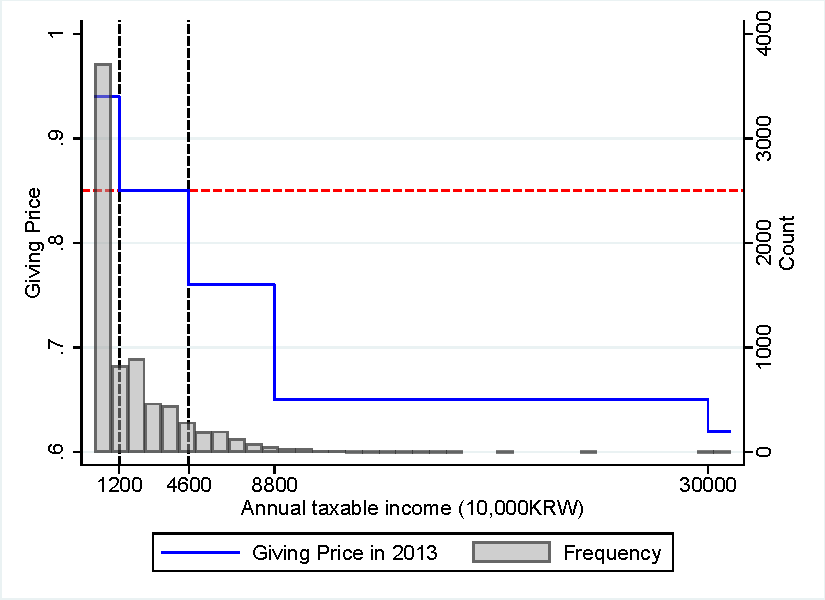
\includegraphics[width=0.9\linewidth]{C:/Users/katoo/Desktop/NASTAB/_assets/SummaryPriceChange} 

}

\caption{Income Distribution and Giving Price in 2013}\label{fig:unnamed-chunk-2}
\end{figure}

\clearpage
\end{frame}

\begin{frame}{References}
\protect\hypertarget{references}{}
\hypertarget{refs}{}
\begin{CSLReferences}{1}{0}
\leavevmode\hypertarget{ref-Bursztyn2017}{}%
Bursztyn, L., Jensen, R., 2017. Social image and economic behavior in the field: Identifying, understanding, and shaping social pressure. Annual Review of Economics 9, 131--153. doi:\href{https://doi.org/10.1146/annurev-economics-063016-103625}{10.1146/annurev-economics-063016-103625}

\end{CSLReferences}
\end{frame}

\end{document}
